\chapter{Interferometria a retroiniezione}
\label{capitolo2}
\thispagestyle{empty}

\textit{In questo Capitolo verranno trattati i principi di base dell'interferometria, in particolare verrà presentata la tecnica utilizzata dello strumento di misura sviluppato in questo lavoro di Tesi: l'interferometria a retroiniezione. Dopo aver descritto il principio di funzionamento dell'interferometria a retroiniezione, saranno esposti i principali vantaggi, svantaggi e limitazioni di questa tecnica. In conclusione, verranno descritti i campi di applicazione della tecnica a retroiniezione ponendo particolare attenzione al campo d'applicazione dello strumento sviluppato: misura di distanza assoluta.}

\section{Principi di interferometria convenzionale}
L'interferometria convenzionale è una tecnica che si basa sulla sovrapposizione di due o più fasci ottici, emessi dalla stessa sorgente, al fine di ottenere una frequenza di battimento (frequenza risultante dalla sovrapposizione) che contiene informazioni sui differenti cammini percorsi dai due fasci. Questa tecnica è in accordo con la teoria ondulatoria della luce che attribuisce alla propagazione della luce le caratteristiche della propagazione delle onde (elettromagnetiche) elastiche. Essa si basa sul fenomeno dell'interferenza e in particolare si sfrutta il principio secondo cui un'onda risultante dalla combinazione di due onde differenti mantiene proprietà che dipendono dalle onde generatrici.

I campi di applicazione di tale tecnica spaziano dall'astronomia alla metrologia ottica. Essa, in generale, trova applicazioni in ambiti dove l'ambiente di lavoro è critico (ad esempio superfici calde) o l'oggetto da misurare è difficilmente raggiungibile.
\begin{figure}  
  \begin{center}
    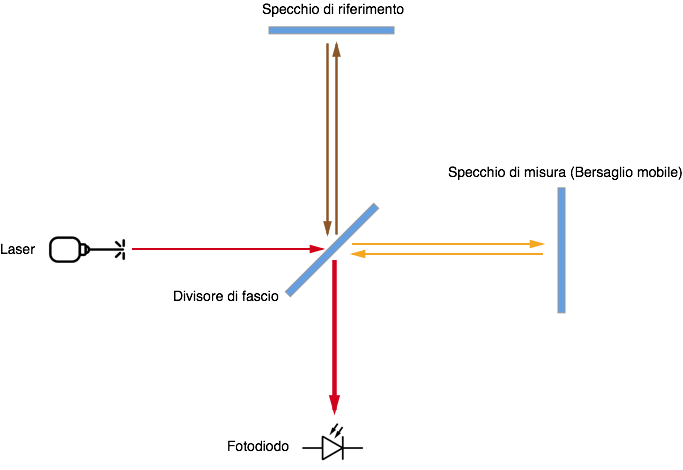
\includegraphics[scale=0.4]{cap2/michelson}
    \caption{Interferometro di Michelson}
    \label{michelson}
  \end{center}
\end{figure}
La configurazione ottica interferometrica classica, mostrata in Figura \ref{michelson}, è definita interferometro di \textit{Michelson}~\cite{sensmeslaser}. Questa configurazione è costituita da una sorgente laser, un divisore di fascio (\textit{beam splitter}), due specchi e un fotodiodo.

Il funzionamento dell'interferometro di Michelson consiste nel duplicare il fascio ottico emesso dalla sorgente laser, tramite uno specchio semiriflettente (divisore di fascio), in due cammini ottici distinti, di cui uno noto (di riferimento) e uno di misura. Entrambi i fasci, vengono riflessi da due specchi posti all'estremità dei due cammini. Lo specchio posto nel ramo di riferimento è fisso, mentre quello posto sul ramo di misura è mobile. Successivamente i fasci di riferimento e di misura vengono sovrapposti e indirizzati, attraverso il \textit{beam splitter}, verso il fotodiodo. Il fascio risultante è la combinazione di due fasci iso-frequenziali, ma sfasati a causa dei diversi cammini percorsi.

Infine, il fotodiodo produce una corrente, proporzionale all'intensitá del fascio laser incidente su di esso, che contiene l'informazione sullo spostamento del bersaglio. Tale corrente fotogenerata è associata alla potenza incidente che è proporzionale alla somma dei campi elettrici dei rispettivi cammini.

Indicando con ${E_m}$ il campo elettrico relativo al cammino di misura e con ${E_r}$ il campo elettrico relativo al cammino di riferimento, la corrente fotogenerata $I_{ph}$ segue la relazione:
\begin{equation}
\begin{split}
	I_{ph}&=\sigma|E_r+E_m|^2=\sigma\{E_r^2+E_m^2+2E_rE_mRe[e^{i(\phi_m-\phi_r)}]\}\\
	&=I_r+I_m+2\sqrt{I_rI_m}\cos{(\phi_m-\phi_r)}
\end{split}
\end{equation}
dove $\sigma$ è il coefficiente di conversione del fotodiodo, $E_r$ e $E_m$ sono rappresentati come vettori rotanti di ampiezza $|E_{m,r}|$ e fase $\phi_{m,r}$ e la terza componente $2\sqrt{I_rI_m}\cos{(\phi_m-\phi_r)}$ costituisce la fase interferometrica. 

Per come é costruito l'interferometro di \textit{Michelson}, si avrà che la fase $\phi_r$ sará sempre costante, mentre quella relativa a $\phi_m$ varierá in funzione dello spostamento dell'ostacolo. Quindi ció che si ottiene sará una corrente fotogenerata che dipenderá dal coseno della fase $\phi_m$. 

Indicando con $k=\frac{2\pi}{\lambda}$ il numero d'onda (numero di oscillazione nell'unità di lunghezza) è possibile esplicitare l'argomento del coseno ottenendo:
\begin{equation}
	\phi=ks=\frac{2\pi}{\lambda}s	
\end{equation}
dove $\lambda$ è la lunghezza d'onda della sorgente laser e $s$ è lo spostamento.

Essendo $\phi_r= ks_r$ e $\phi_m = ks_m$, si può ricavare la variazione di fase totale, ottenendo:
\begin{equation}
	\Delta \phi=\phi_m-\phi_r=k(s_m-s_r)=\frac{2\pi}{\lambda}(s_m-s_r)
\end{equation}
dove $s_m$ e $s_r$ sono rispettivamente i cammini ottici di misura e di riferimento.

La variazione di fase del segnale interferometrico contiene quindi l'informazione sullo spostamento del bersaglio rispetto al cammino di riferimento. Il segnale interferometrico è quindi periodico per sfasamenti totali pari a $2\pi$, che corrispondono ad uno spostamento $s_m$ pari a $\frac{\lambda}{2}$. La misura avviene tramite il semplice conteggio delle frange interferometriche del segnale nel tempo. La risoluzione dello strumento di misura risulta quindi essere pari a  $\frac{\lambda}{2}$.

\subsection{Svantaggi dell'interferometria convenzionale} 
L'interferometro di \textit{Michelson} è molto vantaggioso dal punto di vista della semplicità di realizzazione perché vi è un impiego ridotto di componenti, ma presenta tuttavia notevoli svantaggi nella pratica:
\begin{figure}  
  \begin{center}
    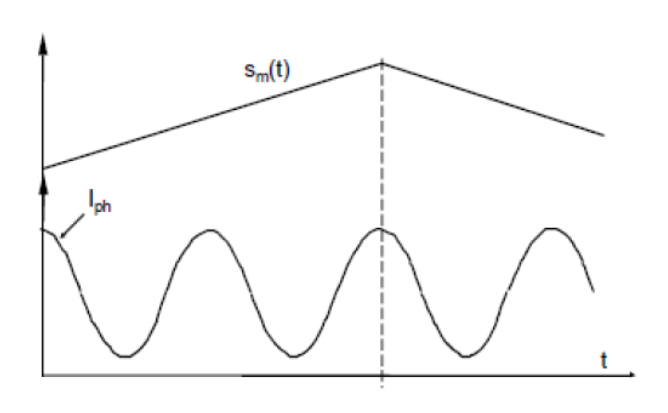
\includegraphics[scale=0.4]{cap2/versospost}
    \caption{Ambiguità sul verso di spostamento}
    \label{versospost}
  \end{center}
\end{figure}
\begin{itemize}
	\item L'allineamento degli specchi, per far convergere i due fasci di luce coerenti nello stesso punto, e il posizionamento del \textit{beam splitter} richiedono accuratezza elevata e sono quindi di difficile realizzazione.
	\item Richiede l'utilizzo di un bersaglio cooperativo e di una particolare ottica di collimazione. Non realizzabile in caso di misura non invasiva.
	\item Non permette di discriminare il verso di spostamento del bersaglio con conseguente ambiguità del movimento misurato. Tale ambiguità è causata dalla risposta cosinusoidale, come mostrato in Figura \ref{versospost}.
	\item La misura subisce alterazioni in caso di retroiniezione non voluta di luce esterna all'interno della cavità ottica del laser.
	\item L'utilizzo di sorgenti laser a gas comporta elevati costi di realizzazione dello strumento.
\end{itemize}
Tutto ciò ha fatto emergere la necessità di uno strumento che presentasse una semplicità di utilizzo e un costo contenuto.

\section{Interferometria a retroiniezione}
È stato esposto, nel paragrafo precedente, come l'interferometria convenzionale presenti notevoli svantaggi. Per tale motivo viene presentata una differente tecnica interferometrica: si tratta dell'interferometria a retroiniezione, chiamata anche interferometria a self-mixing~\cite{1464-4258-4-6-371}.

La tecnica interferometrica a retroiniezione rende possibile la realizzazione di uno strumento di misura tramite il semplice utilizzo di una sorgente laser e di una lente per focalizzare il raggio ottico. Questa configurazione interferometrica risolve, quindi, i problemi dell'interferometria convenzionale, presentando una ridotta complessità di realizzazione e un costo contenuto. Per tale motivo il misuratore realizzato in questo lavoro di tesi sfrutta codesta tecnica.

\begin{figure}  
  \begin{center}
    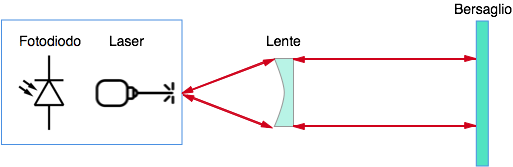
\includegraphics[scale=0.5]{cap2/selfmix}
    \caption{Schema di principio di un interferometro a retroiniezione}
    \label{selfmix}
  \end{center}
\end{figure}

La configurazione base del misuratore a self-mixing è formata da un diodo laser, posto a distanza $s$ dal bersaglio, un'ottica collimatrice e un fotodiodo, che può essere anche quello di monitor integrato nello stesso package del laser. Lo schema base è riportato in Figura \ref{selfmix}.

La modalitá self-mixing, a differenza dell'interferometro convenzionale, non utilizza porzioni di fascio ottico come riferimento. Per effettuare la misura viene sfruttata una porzione di luce riflessa dalla superficie del bersaglio che, rientrando nella cavità laser attraverso la lente, genera un battimento ottico con l'onda laser già presente. La luce riflessa dal bersaglio arriva con verso opposto al precedente cammino e con una potenza che è una frazione di quella emessa, a causa dell'attenuazione data dal tragitto laser-ostacolo-laser.

\'E possibile esplicitare la potenza della luce riflessa dal bersaglio con la relazione:
\begin{equation}
	P_r=\frac{P_0}{A}
\end{equation}
dove $P_0$ è la potenza ottica della radiazione emessa e $A$ è il coefficiente di attenuazione.

All'interno della cavità ottica del laser si verifica un fenomeno di interferenza: il campo elettrico $E_0$ della radiazione emessa si combina con il campo elettrico $E_r$ della luce retroiniettata. Come descritto nel paragrafo precedente, anche in questa situazione, $E_r$ risulta avere uno sfasamento ottico che è pari a:
\begin{equation}
	\phi=2ks
\end{equation}
dove $k=\frac{2\pi}{\lambda}$ è il numero d'onda e $s$ è la distanza.
\begin{figure}  
  \begin{center}
    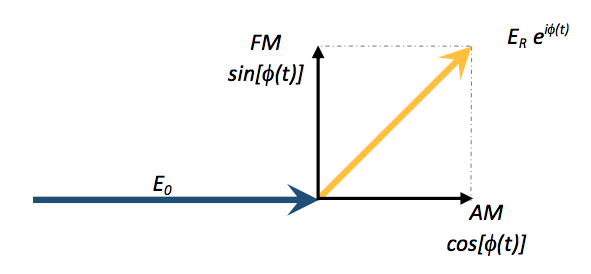
\includegraphics[scale=0.5]{cap2/rapprvet}
    \caption{Rappresentazione vettoriale dell'interferenza all'interno della cavità laser}
    \label{rapprvet}
  \end{center}
\end{figure}
Come mostrato in figura \ref{rapprvet} è possibile scomporre $E_r$, operando un'analisi vettoriale, nelle sue componenti in fase ed in ampiezza. Ciò permette, nella cavità ottica, sia la modulazione in frequenza (FM) che la modulazione in ampiezza (AM) del campo elettrico emesso originariamente dalla sorgente $E_0$. 

La componente che opera la modulazione d'ampiezza è $E_r\cos[\phi(t)]$, mentre la componente di modulazione di frequenza è $E_r\sin[\phi(t)]$. Le' due componenti sono sfasate di $90\degree$ e quindi la discriminazione dei due segnali in quadratura permette di ricavare senza ambiguità il verso dello spostamento del bersaglio, al contrario dell'interferometro di \textit{Michelson}.

L'equazione che governa la corrente nel fotodiodo sará:
\begin{equation}
	I_{ph}=I_0(1+m_{AM})\cos{[(1+m_{FM})\omega t]}
\end{equation}
dove $m_{AM}$ e $m_{FM}$ sono le profondità di modulazione.

Se si utilizza un laser a semiconduttore, come nel caso dello strumento presentato in questa Tesi, la componente FM presente nel fotodiodo é impossibile da estrarre in quanto presenta frequenze dell'ordine delle decine di $MHz$. Quindi, l'unica modulazione visibile sulla corrente del fotodiodo è quella AM:
\begin{equation}
	I_{ph}=I_0(1+m_{AM})\cos{[\omega t]}
\end{equation}
Il funzionamento di un diodo laser a singolo modo longitudinale soggetto a retroiniezione è descritto dalle equazioni differenziali sviluppate da Lang\&Kobayashi~\cite{1070479}; tuttavia, la risoluzione analitica di tali equazioni non è necessaria ai fini di questo lavoro di tesi.

Per questo motivo nel paragrafo successivo è presentata soltanto una soluzione qualitativa delle equazioni di Lang\&Kobayashi, con lo scopo di determinare i regimi di retroiniezione della tecnica self-mixing.

\subsection{Regimi di retroiniezione tramite risoluzione qualitativa}
\begin{figure}  
  \begin{center}
    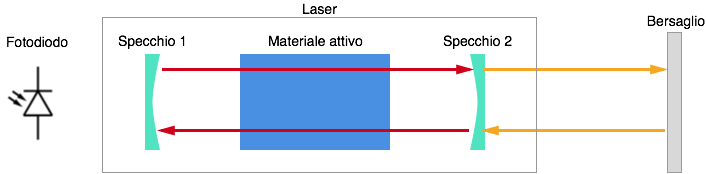
\includegraphics[scale=0.5]{cap2/roundtrips}
    \caption{Round trip ottico del campo elettrico all'interno della cavità laser}
    \label{roundtrips}
  \end{center}
\end{figure}
Un approccio qualitativo per determinare i regimi di retroiniezione è quello di considerare il \textit{round trip} del campo elettrico di Figura \ref{roundtrips}. In figura sono stati evidenziati i \textit{round trip} all'interno della cavità e tra il bersaglio e la cavità stessa.

Il campo elettrico totale presente all'interno della cavità è dato dalla somma di due campi elettrici: quello dovuto alla riflessione dello specchio interno posto al lato opposto della cavità e quello dovuto alla riflessione del bersaglio. Il campo elettrico risultante è quindi:
\begin{equation}
	E'=ER_1R_2e^{2\gamma L}e^{2jkL}+E\alpha e^{2jks}
\end{equation}
dove:
\begin{itemize}
	\item $R_1$ e $R_2$ sono rispettivamente le riflettività dello specchio in cavità e del bersaglio
	\item $\gamma$ è il guadagno netto per unità di lunghezza
	\item $L$ è la lunghezza della cavità
	\item $s$ è la distanza tra il secondo specchio ed il bersaglio
	\item $\alpha$ è il fattore di riflessione (o diffusione) del bersaglio
\end{itemize}

\'E possibile, quindi, ricavare facilmente dall'equazione precedente il guadagno d'anello:
\begin{equation}
	G_{loop}=\frac{E}{E'}=R_1R_2e^{2\gamma L}e^{2jkL}+\alpha e^{2jks}
\end{equation}
Per far si che il sistema sia in grado di produrre oscillazioni spontanee che si mantengano nel tempo con ampiezza costante è necessario rispettare il criterio di \textit{Barkhausen}, il quale afferma che il sistema non deve modificare l'ampiezza del segnale e non deve introdurre sfasamento complessivo. Tali condizioni sono riassunte come segue:
\begin{equation}
	\begin{cases}
   |G_{loop}|=1\\\Phi_{loop} = 0
   \end{cases}
\end{equation}
Per studiare le soluzioni del sistema, si divide l'analisi del problema in due casi:
\begin{enumerate}
	\item In assenza di retroazione 
	\item In presenza di retroazione
\end{enumerate}
Nel primo caso, ovvero con coefficiente $\alpha$ nullo, si trovano le stesse equazioni di un normale laser in cui il guadagno e le perdite sono uguali, ovvero:
\begin{equation}
	\begin{cases}
   G_{loop}=R_1R_2e^{2\gamma L}\\Phi_{loop} = 2kN=N2\pi
   \end{cases}
\end{equation}
con:
\begin{equation}
k=2\pi n_l \frac{\nu_0}{c}	
\end{equation}
\begin{equation}
	\nu_0 = N\frac{c}{2n_lL}
\end{equation}

dove $k$ è il numero d'onda, $\nu_0$ sono i modi di risonanza e $n_l$ rappresenta l'indice di rifrazione del mezzo attivo.

Se la frequenza reale si discosta da quella di risonanza propria, la frazione di fase $2kL$ in eccesso rispetto ad un multiplo di $2\pi$ può essere scritta come:
\begin{equation}
	2kL=4\pi n_l L \frac{\nu - \nu_0}{c}
\end{equation}

\subsection{Vantaggi e svantaggi dell'interferometria a retroiniezione}

\section{Principali limitazioni della tecnica interferometrica}

\section{Applicazioni dell'interferometria a retroiniezione}

\subsection{Misura di distanza assoluta}

\subsection{Velocimetria}